\chapter{Výsledky experimentů}
V této kapitole jsou shrnuty výsledky, kterých bylo v rámci práce na tématu dizertace dosaženo. Jmenovitě jsou to výsledky navrženého algoritmu Extreme Seeking Entropy (viz kapitola \ref{chap: ESE_vysledky}) a potom použití algoritmu Learning Entropy pro adaptivní fuzzy filtr při detekci změn stavu bioprocesu (viz kapitola \ref{chap:LE_fuzzy}).
\section{Výsledky detekce novosti algoritmu Extreme Seeking Entropy}\label{chap: ESE_vysledky}
\#TODO
\subsection{Případová studie: chatociká časová řada Mackey-Glass a detekce pertubace}
\#TODO
\subsection{Případová studie: detekce skokové změny parametrů generátoru signálu}
\#TODO
\subsection{Případová studie: detekce náhlé absence šumu}
\#TODO
\subsection{Případová studie: detekce změny trendu}
\#TODO
\subsection{Případová studie: detekce epilepsie v myším EEG}
\#TODO
\subsection{Vyhodnocení úspěšnosti detekce skokové změny parametrů generátoru signálu}
\#TODO
\subsection{Vyhodnocení úspěšnosti detekce změny trendu a evaluace ROC křivky}
\#TODO
\section{Vyhodnocení výpočetní náročnosti metod odhadu parametrů zobecněného Paretova rozdělení}
Výsledky v této podkapitole byli publikovány v (můj shit).
\subsection{Motivace}
Detekce novosti v reálném čase je úloha, která nalézá své uplatnění nejen v oblasti detekci a diagnostiky v průmyslových aplikacích \cite{fault}, ale také např. v detekci narušení počítačových sítí \cite{data_streams} nebo v zabezpečovacích systémech \cite{surveilance}. Další oblastí uplatnění je např. mobilní robotika, která je specifická tím, že robot má k dispozici pouze limitovaný výpočetní výkon \cite{robotics_marslan,robotics}. Pro metody detekce novosti v reálném čase je tedy důležité, aby vynikali dostatečně nízkou výpočetní náročností. Z tohoto důvodu byli otestovány tři různé metody výpočtu parametrů GPD (viz kapitola \ref{chap:gpd}, protože tento výpočet je z hlediska použití algoritmu ESE potenciálně limitující z hlediska využitelnosti v aplikacích detekce v reálném čase. Jmenovitě byli otestovány tyto metody: metoda maximální věrohodnosti (ML), metoda momentů (MOM) a metoda kvazi-maximální věrohodnosti (QML) (více viz kapitola \ref{chap:gpd}). Výpočetní čas potřebný k určení parametrů GPD pomocí těchto metod byl vyhodnocen při experimentu, ve kterém dojde ke skokové změně parametrů generátoru signálu.
\subsection{Specifikace experimentu}
Vzhledem k povaze experimentu, který slouží k vyhodnocení výpočetní náročnosti různých metod určení parametrů GPD, a nikoliv k detekci novosti v nějakém komplexním procesu, byl zvolen jednoduchý lineární kombinační filtr (LNU), jehož výstup v diskrétním časovém okamžiku $k$ je definován jako
\begin{equation}
\hat{y}(k)=w_1\cdot x_1(k)+w_2\cdot x_2(k)+w_3\cdot x_3(k)
\end{equation}
a tento filtr je adaptován algoritmem NLMS (viz kapitola \ref{chap:nlms}), přičemž rychlost učení $\mu$ byla nastavena jako $\mu=0.8$.
\par 
Pro výstup generátoru signálu platí vztah
\begin{equation}
y(k)=x_1(k)+x_2(k)+x_3(k)+v(k)
\end{equation}
pro všechny $1 \leq k \leq 200$. Člen $v(k)$ reprezentuje aditivní gaussovský šum s nulovou střední hodnotou a směrodatnou odchylkou $\sigma_{noise}=0.1$. V diskrétním časovém okamžiku $k=201$ dojde ke změně generátoru signálu a jeho výstup přejde do tvaru
\begin{equation}
y(k)=0.7\cdot x_1(k)+1.2\cdot x_1(k)+1.1 \cdot x_1(k) + v(k)
\end{equation}
pro $201 \leq k \leq 400$. Hodnota všech vstupů generátoru signálu je v každém časovém okamžiku $k$ vybrána ze standartního rozdělení normálního rozdělení, takže $i$-tý vstup $x_i\sim \mathcal{N}(0,1)$. Změna parametrů signálu byla vybrána tak, aby nedošlo ke změně střední hodnoty signálu $y(k)$.
\par
Experimenty byly provedeny na PC s procesorem Intel(R) Core(TM) i5-7400 se 4mi jádry s taktovací frekvencí 3001 MHz a operační pamětí o velikosti 32 GB. Operační systém byl Windows 10 Pro, 64-bitová verze 10.0.18362. Kód byl napsán v Python 3.6.1 a byly použity knihovny Numpy 1.17.0 a Scipy 1.4.1.

\begin{figure}[h!]
	\label{fig:par_output}
	\centering
	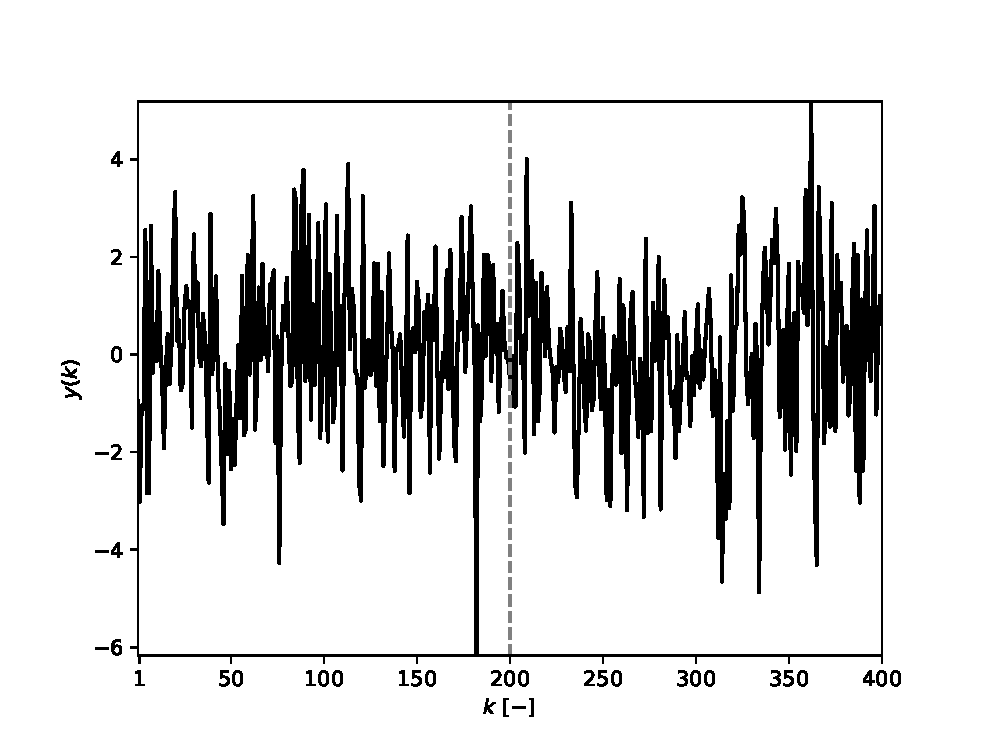
\includegraphics[scale=0.71]{IMG/appel_par/par_output.eps}
	\caption{Výstup adaptivního filtru během experimentu. Skoková změna parametrů generátoru signálu je zvýrazněná svislou vodorovnou čarou v diskrétním časovém okamžiku $k=200$.}
\end{figure}

\subsection{Výsledky a diskuze}


\begin{figure}[h!]
	\label{fig:par_ese}
	\centering
	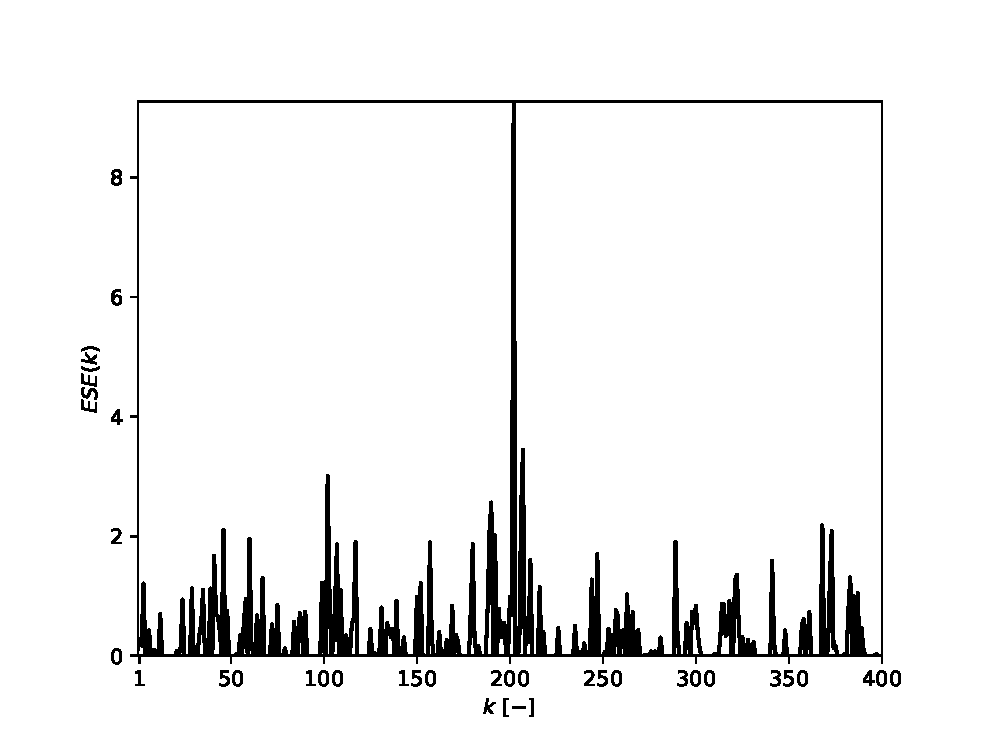
\includegraphics[scale=0.71]{IMG/appel_par/par_ese.eps}
	\caption{Hodnota ESE během experimentu. Globální maximum odpovídá změně parametrů generátoru signálu, resp. úspěšné detekci novosti.}
\end{figure}

\begin{figure}[h!]
	\label{fig:par_mu}
	\centering
	\includegraphics[scale=0.71]{IMG/appel_par/par_mu.eps}
	\caption{Hodnota parametru $\mu$ GPD pro všechny tři adaptivní váhy $w_1$, $w_2$, $w_3$ během experimentu detekce změn parametrů generátoru signálu. Svislá čára v diskrétním časovém okamžiku $k=200$ znázorňuje skokovou změnu parametrů generátoru signálu.}
\end{figure}

\begin{figure}[h!]
	\label{fig:par_gamma}
	\centering
	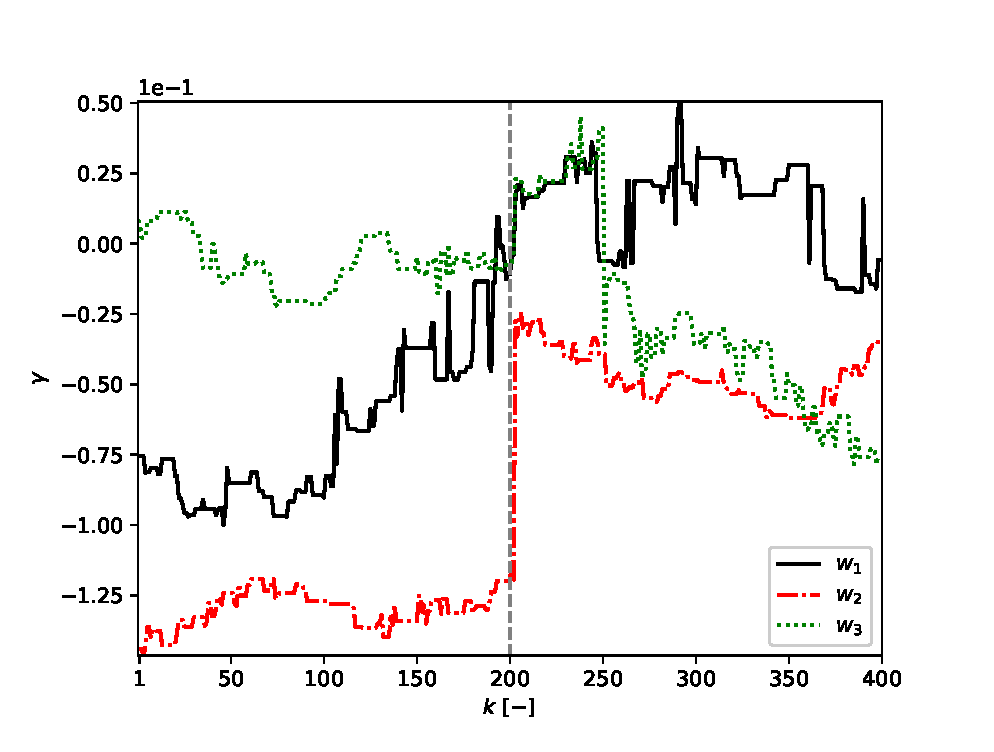
\includegraphics[scale=0.71]{IMG/appel_par/par_gamma.eps}
	\caption{Hodnota parametru $\gamma$ GPD pro všechny tři adaptivní váhy $w_1$, $w_2$, $w_3$ během experimentu detekce změn parametrů generátoru signálu. Svislá čára v diskrétním časovém okamžiku $k=200$ znázorňuje skokovou změnu parametrů generátoru signálu.}
\end{figure}

\begin{figure}[h!]
	\label{fig:par_sigma}
	\centering
	\includegraphics[scale=0.71]{IMG/appel_par/par_mu.eps}
	\caption{Hodnota parametru $\sigma$ GPD pro všechny tři adaptivní váhy $w_1$, $w_2$, $w_3$ během experimentu detekce změn parametrů generátoru signálu. Svislá čára v diskrétním časovém okamžiku $k=200$ znázorňuje skokovou změnu parametrů generátoru signálu.}
\end{figure}
Průměrný čas výpočtu $\overline{t}$ parametrů všech tří GPD (počet GPD odpovídá počtu adaptivních parametrů filtru) a odpovídající směrodatné odchylky $\sigma_t$ jsou uvedeny v následující tabulce \ref{tab:par_results}.
\begin{table}[h]

\centering
\caption{Tabulka průměrných časů výpočtu pro jednotlivé adaptivní váhy a odpovídajících směrodatných odchylek vybraných metod výpočtu parametrů GPD}
\begin{tabular}{|l|l||l|l|}
\hline
 & Metoda & $\overline{t}$ {[}ms{]} & $\sigma_t$ {[}ms{]} \\ \hline \hline
\multirow{3}{*}{$w_1$} & ML & $26.198$ & $3.396$ \\ \cline{2-4} 
 & QML & $0.354$ & $0.478$ \\ \cline{2-4} 
 & MOM & $\textbf{0.076}$ & $0.264$ \\ \hline
\multirow{3}{*}{$w_2$} & ML & $26.718$ & $2.302$ \\ \cline{2-4} 
 & QML & $0.337$ & $0.471$ \\ \cline{2-4} 
 & MOM & $\textbf{0.064}$ & $0.244$ \\ \hline
\multirow{3}{*}{$w_3$} & ML & $24.982$ & $1.964$ \\ \cline{2-4} 
 & QML & $0.395$ & $0.489$ \\ \cline{2-4} 
 & MOM & $\textbf{0.060}$ & $0.238$ \\ \hline

\end{tabular}
 \label{tab:par_results}
\end{table}

Z uvedených výsledků je patrné, že nejrychlejší metoda je MOM. Podstatnou nevýhodou této metody pro využití v aplikacích, které vyhodnocují data v reálném čase je její omezení na hodnoty parametrů GPD (viz kapitola \ref{chap:gpd}). Pokud parametry uvedené omezení nesplňují, vypočtené hodnoty nepřesné (resp. nesmyslné) a tedy nepoužitelné pro algoritmus ESE, který začne produkovat nepřesné výsledky. Z pohledu úlohy detekce novosti je diskutabilní, zda-li můžeme garantovat, že sledovaný proces po celou dobu bude splňovat uvedené omezení.
\par
Metoda, jejíž výpočetní čas byl nejvyšší je ML, což je vzhledem k iterativnímu nalezení parametrů GPD očekávatelné. Jednou z nevýhod použití této metody je nemožnost určit minimální a maximální počet iterací. Jednou z možností jak zrychlit nalezení parametrů je využití apriorní informace o hodnotách těchto parametrů. V rámci experimentu však byla využita pouze apriorní informace o parametru $\mu$, který odpovídá nejmenší hodnotě přírůstku vah v okně.






\section{Případová studie použití algoritmu Learning Entropy a adaptivního fuzzy filtru pro detekci změn stavů bioprocesu} \label{chap:LE_fuzzy}
\#TODO
\subsection{Popis bioprocesu a specifikace problému}
Podle \cite{fermentace} je pro fermentační procesy, které probíhají v dávkovém režimu je podstatné, aby probíhalo správně dávkované živení substrátem. Pro tyto procesy je specifické, že se při nadměrných koncentracích stává substrát pro mikroorganismy toxickým a může dojít k tzv. přeživení a tím i zahubení těchto mikroorganismů. Naopak, v důsledku nedostatečného zábovení živinami může dojít k odumření kultivovaného organismu. Z tohoto pohledu se je tedy důležité v závislosti na koncentraci substrátu a stavu populace mikroorganismů měnit i strategii pro řízení procesu kultivace. Historicky byl stav bioprocesu klasifikován expertem, přičemž vyhodnocení bylo poměrně časově náročné a nebylo neobvyklé, že různí experti docházeli k rozdílným závěrům. Protože výnos fermentačního procesu je zásadním způsobem ovlivněn správnou klasifikací stavu ve kterém se právě nacházi, bylo by vhodné klasifikaci automatizovat a pokud možno zvýšit její přesnost. Tomuto problému je právě věnována publikace \cite{fermentace}, která řeší problém automatické klasifikace stavů bioprocesu kultivace bakterie \textit{Pseudomonas putida KT2442}. V této publikaci je navržen komplexní algoritmus pro online klasifikaci stavů bioprocesu. Autoři zde rozlišují celkem tři stavy bioprocesu kultivace \textit{Pseudomonas putida KT2442}, konkrétně:
\begin{enumerate}
    \item normální živení
    \item přeživení
    \item nedoživení
\end{enumerate}
Navržený algoritmus vyhodnocuje přísun vstupujících živin (Fm), respektive substrátu, a změny a trendu rozpuštěného kyslíku (DO), který je produkován bakteriemi \textit{Pseudomonas putida} a pomocí hřebenové regrese (v literatuře se vyskytuje také pod názvem Tichonova regularizace) je určován vývoj populace bakterií respektive stav bioprocesu. Vzhledem k tomu, že modely vývoje populace pro jednotlivé stavy jsou různé, mohlo by v průběhu experimentu dojít i k podstatným změnám v adaptivním modelu v okamžicích změn stavů kultivace. Tyto změny se mohli projevit neobvykle velkými přírůstky adaptivních parametrů. 
\par
Protože algoritmus Learning Entropy využívá přírůstku adaptivních parametrů, mohl by být vhodným nástrojem pro detekci změn stavů bioprocesu. Předpokládáme, že tedy existuje korelace mezi změnami stavu bioprocesu a nárůstem Learning Entropy. Přestože může být proces kultivace bakterií \textit{Pseudonomas Putidas} modelován různými a různě složitými modely, pro využití algoritmu Learning Entropy se jeví výhodné použít jednoduché prediktory nebo sledovače. Dosud publikované články využívali pro algoritmus LE pouze FIR filtry, případně Volterrovy filtry, které mají adaptivní parametry v lineární závislosti. V tomto experimentu je použit adaptivní fuzzy filtr, jehož struktura je specifikována v kapitole \ref{chap:fuzzyf} a k jehož adaptaci byl použit algoritmus, který je uveden v kapitole \ref{chap:gd}.
\par
Použitý adaptivní fuzzy filtr má 9 pravidel ($M=9$), jehož $l$-té pravidlo je ve tvaru
\begin{equation}
    IF\;do(k-1)\; is\; A_1^l\;AND\;do(k-6)\;is\;A_2^l\;AND\;do(k-19)\;is\;A_3^l\;THEN\;do(k)\;is\;B^l
\end{equation}
kde $A_i^l$ je množina ve vstupním prostoru $U \subset R^3$ a $B^l$ je fuzzy množina ve výstupním prostoru $V \subset R$. V uvedeném pravidle jsou $do(k-1)$, $do(k-6)$, $do(k-19)$ a $do(k)$ lingvistické proměnné, které vyjadřují koncentraci rozpuštěného kyslíku $do$ v v diskrétních časových okamžicích $k$, $k-1$, $k-6$ respektive $k-19$, kde $k$ je diskrétní časový index. Vzhledem k tomu, že uvedený adaptivní fuzzy filtr používá Gaussovské funkce příslušnosti (viz kapitola \ref{chap:fuzzyf} je zobrazení popisující jeho výstup ve tvaru
\begin{equation}
    \hat{y}(\textbf{x}(k))=\frac{\sum_{j=1}^9 \overline{b}^j\Big[\prod_{i=1}^3 exp\Big(-\Big(\frac{x_i-\overline{x}_i^j}{\sigma_i^j}\Big)\Big)\Big]}{\sum_{j=1}^9 \Big[\prod_{i=1}^3 exp\Big(-\Big(\frac{x_i-\overline{x}_i^j}{\sigma_i^j}\Big)\Big)\Big]}
\end{equation}
kde vektor $\textbf{x}(k)$ je
\begin{equation}
    \textbf{x}(k)=[do(k-1),do(k-6),do(k-19)].
\end{equation}\
Protože hodnota koncetnrace rozpuštěného kyslíku je uváděna v procentech, platí pro všechna $x_i\in \langle 0;100\rangle$. K adaptování výše uvedeného filtru byl použit algoritmus gradient descent (viz kapitola \ref{chap:gd}. Maximální počet epoch byl stanoven na $q_{max}=100$ a požadovaná chyba predikce mezi výstupem adaptivního filtru a naměřenými daty na $\epsilon=0,001$. Rychlost učení byla během experimentů nastavena na $\mu=1$.
\par
Pro vyhodnocení novosti byla použita přímá verze algoritmu LE, takže
\begin{equation}\label{eq:le_putida}
    E(k)=max\{0, \sum_{j=1}^9 z(\abs{\Delta \overline{b^j})}-\beta\}
\end{equation}
kde funkce $z$ je dána rovnicí (XY) a $\beta$ je citlivostní parametr. Pro vyhodnocení novosti jsou tedy použity změny polohy středů množin ve výstupním prostoru, nikoliv změny parametrů fuzzy množin ve vstupním prostoru.

\subsection{Experiment a zhodnocení}
Experiment s použitím algoritmu LE a adaptivního fuzzy filtru byl uskutečněn na datech z kultivace bakterie \textit{Pseudonomas Putida}, který byl uskutečněn na Ústavu počítačové a řídicí techniky VŠCHT Praha. Celkem byly zpracovávány hodnoty ze dvou kultivací. Přestože bylo během experimentu měřena sada různých veličin (např. teplota, pH, atd.), osvědčil se pro použití LE signál rozpustěného kyslíku $do$ $[\%]$. Během experimentu bylo použito vzorkování $T=1$ $min$, což je vzhledem k rychlosti celého procesu dostatečně rychlé vzorkování. Počáteční nastavení parametrů adaptivního fuzzy filtru bylo provedeno tak, jak je popsáné v kapitole \ref{chap:gd}. Podstatný vliv na výsledek detekce změn stavu bioprocesu měla volba volba délky okna pro vyhodnocení změn adaptabilních parametrů filtru $M_{ND}$. Na základě experimentů s různými délkami byla nakonec zvolena délka okna $M_{ND}=20$.
\par
Na následujících obrázcích je znázorněn průběh signálu $do$ během první kultivace (viz obrázek \ref{fig:artep_1}), chyba predikce (viz obrázek \ref{fig:artep_3}) a odpovídající hodnoty $LE$ společně se stavy bioprocesu (viz obrázek \ref{fig:artep_4}). Význam stavů bioprocesu znázorněných na obrázku \ref{fig:artep_3} respektive obrázku \ref{fig:artep_6} jsou: 1 - nedoživení, 2 - živení, 3 - přeživení. Aby byli detekovány všechny změny stavu bioprocesů, byla stanovena hodnota parametru $\beta=2,58$ (viz rovnice \ref{eq:le_putida}).
\par
Data z druhé kultivace byla použita k ověření správného nastavení parametru $\beta$.  Obrázek \ref{fig:artep_2} zobrazuje průběh signálu $do$ během druhého experimentu. Chyba predikce adaptivního fuzzy filtru je zobrazena na obrázku \ref{fig:artep_5}.  Obrázek \ref{fig:artep_6} zobrazuje stavy bioprocesu během kultivace a odpovídající hodnoty $LE$. S tímto nastavením parametru $\beta$ se podařilo detekovat pouze tři změny bioprocesu. Nicméně pro jiné hodnoty délky okna $M_{ND}$ a hodnoty parametru $\beta$ se tyto změny detekovat podařilo. Je tedy zřejmé, že pro praktické použití je správná volba obou parametrů zásadní. Vzhledem k malému množství dat a časové náročnosti kultivace nebylo možné použít nějakou validační metodu. 

\begin{figure}
    \centering
    \includegraphics[scale=0.8]{IMG/artep/artep17_1.png}
    \caption{Průběh signálu $do$ během první kultivace}
    \label{fig:artep_1}
\end{figure}

\begin{figure}
    \centering
    \includegraphics[scale=0.8]{IMG/artep/artep17_3.png}
    \caption{Chyba predikce $e$ během první kultivace}
    \label{fig:artep_3}
\end{figure}

\begin{figure}
    \centering
    \includegraphics[scale=0.8]{IMG/artep/artep17_4.png}
    \caption{Stav bioprocesu a hodnota $LE$ první kultivace}
    \label{fig:artep_5}
\end{figure}

\begin{figure}
    \centering
    \includegraphics[scale=0.8]{IMG/artep/artep17_2.png}
    \caption{Průběh signálu $do$ během druhé kultivace}
    \label{fig:artep_2}
\end{figure}

\begin{figure}
    \centering
    \includegraphics[scale=0.8]{IMG/artep/artep17_5.png}
    \caption{Chyba predikce $e$ během druhé kultivace}
    \label{fig:artep_4}
\end{figure}

\begin{figure}
    \centering
    \includegraphics[scale=0.8]{IMG/artep/artep17_6.png}
    \caption{Stav bioprocesu a hodnota $LE$ během druhé kultivace}
    \label{fig:artep_6}
\end{figure}




 